\chapter*{Preamble}
\marginnote{Stitz-Zeager [\url{www.stitz-zeager.com}] and Boundless [\url{www.boundless.com}] are good backgrounds references.}

The point of these notes is to introduce the main concepts of calculus using what is known as little-$o()$ notation, in the hope to provide a perspective that is simple, expressive, intuitive and correct.

\section*{Algebra is essential}
\begin{marginfigure}
\begin{center}
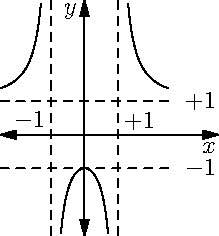
\includegraphics[width=0.75\linewidth]{graphics/algebra1.pdf}
\end{center}
\caption{$y=f(x)=\frac{x^2+1}{x^2-1}$}
\label{fig:algebra1}
\end{marginfigure}
\begin{marginfigure}
\begin{center}
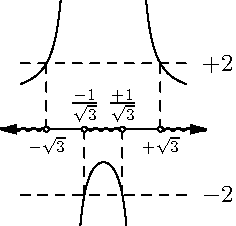
\includegraphics[width=0.75\linewidth]{graphics/algebra2.pdf}
\end{center}
\caption{Where $|f(x)|$ is less than $2$.}
\label{fig:algebra2}
\end{marginfigure}
\begin{marginfigure}
\begin{center}
\includegraphics[width=0.75\linewidth]{graphics/explog.pdf}
\end{center}
\caption{How $y=e^x$ and $x=\ln y$ are related, where $e \approx 2.72$ is Euler's constant.}
\label{fig:explog}
\end{marginfigure}

I assume you are comfortable with algebra, including working with rational algebraic expressions, exponents and logarithms, function notation, absolute values, and inequalities.

For example, seeing 

\begin{equation*}
f(x)=\frac{x^2+1}{x^2-1}
\end{equation*}

And being asked to show
\begin{equation*}
    f(x+h)=\frac{x^2+1}{x^2-1}+ \frac{2h\cdot(2x+h)}{(x-1)(x+1)(x+h+1)(x+h-1)}
\end{equation*}
and
\begin{align*}
  |f(x)|<2 & \text{ if and only if } \\
           &  x \in (-\infty,-\sqrt{3})\cup(-\frac{1}{\sqrt{3}},+\frac{1}{\sqrt{3}})\cup(+\sqrt{3},+\infty)
\end{align*}
should seem (at worst) tedious, but not mysterious.  Neither should the following\footnote{Recall $b^x=e^{x \ln b}$ and $\log_b x=\ln x/\ln b$}:
\begin{equation*}
    2^{\log_3(x)}=x^{\log_2(3)} \,.
\end{equation*}

If these are mysterious to you, then you need to learn college algebra.
\newpage\section*{Trigonometry is helpful}
\begin{marginfigure}
\begin{center}
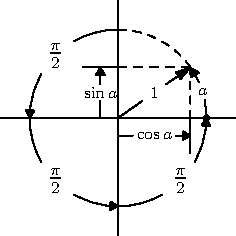
\includegraphics[width=0.75\linewidth]{graphics/unitcircle.pdf}
\end{center}
\caption{Defining $\cos a$ and $\sin a$ for radian angle $a$ on the unit circle. Notice there are $2\pi \approx 6.28$ radians in a circle.}
\label{fig:unitcircle}
\end{marginfigure}
It will be useful if you have some basic trigonometry, including measuring angles in radians, which is the only unit of angle we care about here.  For example,
\begin{gather*}
    (\cos a)^2 +(\sin a)^2 = 1\,,\\
    \cos a=
        \frac{1}{2}\text{ if and only if $a=\pm\frac{\pi}{3}+2\pi n$, for some integer $n$}\,,
\intertext{and}
    \sin(a \pm b)=\sin(a) \cos(b) \pm \cos(a) \sin(b)\,, \\
    \cos(a \pm b)=\cos(a) \cos(b) \mp \sin(a) \sin(b)\,, \\
\end{gather*}
should at least be familiar to the point of looking something up to remember the details.

\begin{marginfigure}
\begin{smallsudoku} % -- simple
| | |6|1| |5| | | |.
|9| | | |4| |7| | |.
|8| | |7| | | |2| |.
|4| | | | | | | | |.
| | |1| | | |4| | |.
| | | | |6| | | | |.
| |5| |8| |2|1| | |.
| |6| | | |9| | |7|.
| |4| | | |6|9| |5|.
\end{smallsudoku}
\caption{A simple sudoku puzzle.  Each row, column and $3 \times 3$ subgrid must contains all of the digits from 1 to 9.}
\label{fig:sudoku-simple}
\end{marginfigure}
\section*{Reading Tips}
\begin{marginfigure}
\begin{center}
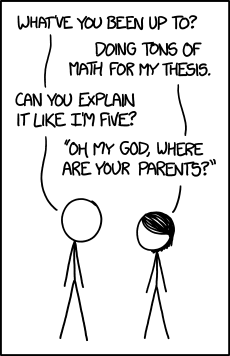
\includegraphics{graphics/like_im_five.png}
\end{center}
\caption{\url{http://xkcd.com/1364}}
\label{fig:xkcd1364}
\end{marginfigure}
\begin{itemize}
\item Focus. The best environment for learning something mathematical is in a small group willing to help you work out a sudoku puzzle.  If you can work out a sudoku puzzle in the place and with the people you study with, it is a good sign you can learn math as well.  Learning, any learning, is for mono-taskers: you might multitask (usually poorly) on things you already understand.  This, however, is something you are trying to understand.
\item Drive, don't walk. Learning to use a computer algebra system (like Wolfram Alpha, wxMaxima or Maple), or at least a spreadsheet (like Google Docs, Libre Office or Microsoft Excel) can spare you from a lot of tedium compared to a crummy calculator.
\item Understand first. Proofs are less important than understanding.  If you are mostly interested in applications, don't worry as much about understanding every proof.  Concentrate instead on why the ideas make sense and how you might use these ideas.  If you are interested in mathematics itself, understanding the proofs is important, but useless without an intuition of why they make sense and how to use them.
\end{itemize}
